\documentclass[11pt]{article}
%\renewcommand{\thesection}{\Roman{section}}  %zmiana section na rzymskie
\usepackage[utf8]{inputenc}
\usepackage[OT4]{polski}
\usepackage{tabularx}
\usepackage[margin=60pt]{geometry}
\usepackage{amsmath}
\usepackage{amsfonts}
\usepackage{listings} 
\usepackage[usenames,dvipsnames,table,xcdraw]{xcolor}
\usepackage{array}
\usepackage{sidecap} %do grafik
\usepackage{wrapfig} % j. w.
\usepackage{graphicx} %j.. w.
\usepackage{subfig} %j. w.
\usepackage{booktabs}
\usepackage{longtable}
\usepackage{hyperref}
\usepackage{multirow}



\title{Symulacja komputerowa ruchu ciała w układzie z więzami.}

\author{Paweł Rzońca}

\begin{document}

\maketitle

\section*{Wstęp}
Rozwiążemy problem poruszania się punktu materialnego po powierzchni stożka o kącie 
rozwarcia $2\alpha$ (rys. \ref{r1}) położonego na poziomej płaszczyźnie. 
\begin{figure}[h!]
\begin{center}
\includegraphics[scale=0.8]{rys.png}
\caption{Ilustracja sytuacji} \label{r1}
\end{center}
\end{figure}


Funkcja Lagrange'a w takim przypadku, przy założeniu więzu $r=z$tg$\alpha$, ma postać
\begin{equation}
	\mathcal{L} = \dfrac{1}{2} \left( \mbox{tg}^2\alpha z^2 \omega^2 +
		\dfrac{1}{\cos^2\alpha}v^2 \right) - gz\sin\alpha (1-\cos\varphi),
\end{equation}
gdzie $\omega=\dot{\varphi}$ oraz $v=\dot{z}$. Wykonując odpowiednie óżniczkowania otrzymujemy 
następujące równania ruchu
\begin{equation}\label{1}
\ddot{\varphi} = -\dfrac{g\cos^2\alpha}{\sin\alpha} \dfrac{\sin\varphi}{z} -\dfrac{2\dot{z}\dot{\varphi}}{z}
\end{equation}\label{2}
\begin{equation}
\ddot{z} = \sin^2 \alpha z\dot{\varphi}^2 - g\sin\alpha \cos^2\alpha(1-\cos \varphi).
\end{equation}
Energię całkowitą układu definiujemy przez
\begin{equation}
E=\dot{\vec{q}} \cdot \dfrac{\partial \mathcal{L}}{\partial \dot{\vec{q}}} - \mathcal{L},
\end{equation}
gdzie $\dot{\vec{q}}$ jest prędkością uogólnioną. W tymże układzie 
\begin{equation}
	E = \dfrac{1}{2} \left( \mbox{tg}^2\alpha z^2 \omega^2 +
		\dfrac{1}{\cos^2\alpha}v^2 \right) + gz\sin\alpha (1-\cos\varphi).
\end{equation}
\section*{Metodyka}
Aby rozwiązać układ równań \ref{1} i \ref{2} drugiego stopnia przerabiamy go na układ czterech równań
pierwszego stopnia wprowadzając prędkości. Otrzymujemy:\\
\\
$
\dot{\varphi}=\omega
$\\
$
\dot{z}=v
$\\
$
\dot{\omega}=-\dfrac{g\cos^2\alpha}{\sin\alpha}\dfrac{\sin\varphi}{z} - \dfrac{2v\omega}{z}
$\\
$
\dot{v}=\sin^2\alpha z \omega^2 -g\sin\alpha \cos^2\alpha(1-\cos\varphi)
$\\
$ $\\
W programie podajemy parametr $\alpha$ oraz warunki początkowe. W kolejnych chwilach czasu
liczymy iteracyjnie:\\
$ \omega_{i+1}=\omega_i-\left( \dfrac{g\cos^2\alpha}{\sin\alpha} \dfrac{\sin\varphi_i}{z_i}
+\dfrac{2v_i\omega_i}{z_i}\right)\Delta t$\\
$ v_{i+1} = v_i + \left[ \sin^2\alpha z_i \omega_i^2 -g\sin\alpha\cos^2\alpha (1-\cos\alpha )\right]\Delta t$\\
$ \varphi_{i+1} = \varphi_i +\omega \Delta t$\\
$ z_{i+1} = z_i + v\Delta t$\\
$ t_{i+1} = t_i + \Delta t $
\section*{Wyniki}
Dla ustalenia odpowiedniego kroku czasowego zbadano wykresy \ref{wyk1} energii całkowitej układu od czasu.
Energia ta powinna być stała. Dla kroku czasowego $\Delta t = 0,0001$ s warunek ten jest dobrze spełniony i ten
krok wybrano do symulacji.

\begin{figure}[h!]
\centering
\includegraphics[]{E.eps}
\caption{Wykres energii całkowitej układu w funkcji czasu dla różnych $\Delta t$.
	Pozostałe parametry: $\alpha = 0,5$, $\varphi_0=1,1$, $\omega_0=0 $ rad/s, $z_0=1$ m, $v_0=0 $ m/s.}{\label{wyk1}}
\end{figure}

Sporządzono wykresy przedstawiające zależność $\varphi$ oraz $z$ od czasu dla różnych kątów rozwarcia 
stożka~[\ref{wyk23}] oraz prędkości [\ref{wykV} i \ref{wyko}]. 

Można zauważyć, iż ze wzrostem kąta rozwarcia stośka $2\alpha$ szybkość zmian współrzędnej $\varphi$ maleje.
Natomiast dla współrzędnej $z$ obserwujemy, iż najstromsze nachylenie występuje dla $\alpha$ pośredniego. 
Można spodziewać się, że istnieje tutaj taki kąt, dla którego cząstka najszybciej oddala się od wierzchołka 
stożka. Wyznaczono, iż dla warunków początkowych $\varphi_0=1,1$, $\omega_0=0 $ rad/s, $z_0=1$ m, $v_0=0 $ m/s, kąt 
ten wyniso około $0.621$. Jego wartość zmienia przy zmianie warunków początkowych.

%\footnote{Wartość znaleziona dzięki analizie wielkości $z$ w określonym czasie (10s) 
%dla różnych kątów \ref{aneks}}.
\begin{figure}[h!]
\begin{center}
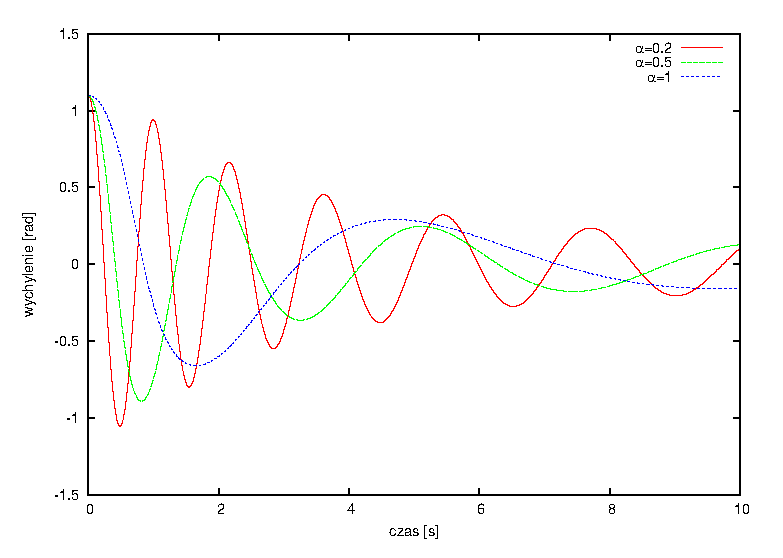
\includegraphics[]{oda.eps}
\includegraphics[]{odam.eps}
\caption{Zależność trajektorii dla różnych wartości parametru $\alpha$.
	Pozostałe parametry: $\varphi_0=1,1$, $\omega_0=0 $ rad/s, $z_0=1$ m, $v_0=0 $ m/s.}{\label{wyk23}}
\end{center}
\end{figure}

\begin{figure}[h!]
\begin{center}\subfloat[$v_0=-1,5$ m/s]{\label{VVV}
\includegraphics[width=0.5\textwidth]{VV-05.png}}
\quad
\subfloat[$v_0=0$ m/s]{\label{odnosnik}
\includegraphics[width=0.5\textwidth]{VV0.png}}
\quad
\subfloat[$v_0=1,5$ m/s]{\label{QQQ}
\includegraphics[width=0.5\textwidth]{VV05.png}}
\caption{Zależność trajektorii dla różnych wartości parametru $v_0$. Położenie $z$ przedstawione jest kolorem
	zielonym, natomiast wychylenie $\varphi$ kolorem czerwonym.
	Pozostałe parametry: $\alpha=0,2$, $\varphi_0=1,1$, $\omega_0=0 $ rad/s, $z_0=3$ m.}{\label{wykV}}

\end{center}
\end{figure}
\begin{figure}[h!]
\begin{center}
\subfloat[$\omega_0=-2$ rad/s]{\label{ZZZ}
\includegraphics[width=0.5\textwidth]{Omega-2.png}}
\quad
\subfloat[$\omega_0=0$ rad/s]{\label{odnosnik}
\includegraphics[width=0.5\textwidth]{Omega0.png}}
\quad
\subfloat[$\omega_0=2$ rad/s]{\label{WWW}
\includegraphics[width=0.5\textwidth]{Omega2.png}}
\caption{Zależność trajektorii dla różnych wartości parametru $\omega_0$. Położenie $z$ przedstawione jest kolorem
	zielonym, natomiast wychylenie $\varphi$ kolorem czerwonym.
	Pozostałe parametry: $\alpha=0,5$, $\varphi_0=1,1$, $v=0 $ m/s, $z_0=5$ m.}{\label{wyko}}
\end{center}
\end{figure}
\newpage
Patrząc na wykresy $z=z(t)$ dla niezerowych prędkości początkowych można zauważyć podobieństwo 
dla krótkich $t$ pomiędzy wykresami \ref{VVV} i \ref{WWW} oraz \ref{ZZZ} i \ref{QQQ}. W rozpatrywanych przpadkach przy odpowiednio długim
czasie, ciało oddala się od czubka stożka, a oscylacje współrzędnej $\varphi$ zmniejszają swoją amplitudę.
\section*{Podsumowanie}
Numeryczne rozwiązanie tego problemu pozwala nam określić trajektorię po jakiej porusza się ciało. W początkowej 
fazie ruchu układ jest bardzo wrażliwy na warunki początkowe. Mimo to w każdym z symulowanych przypadków, po pewnym czasie
ciało porusza się wsdłuż osi $z$ z pewną, w przybliżeniu stałą prędkością, a wachania $\varphi$ stają się mniejsze (ale nie znikają).
Ponadto zaobserwowano, iż szybkość oddalania się od czubka stożka nie zależy w sposób monotoniczny od kąta rozwarcia.



%\section*{Aneks}
%
%\begin{figure}[h!]
%\begin{center}\label{aneks}
%\includegraphics[scale=0.7]{xx.png}
%\caption{Zależność $z=z(10$s$)$ w funkcji kąta $\alpha$.
%	Warunki początkowe: $\varphi_0=1,1$, $\omega_0=0 $ rad/s, $z_0=1$ m, $v_0=0 $ m/s.}
%\end{center}
%\end{figure}

\end{document}


